\documentclass[11pt]{article}
\usepackage{amsmath,amssymb,amsthm}
\usepackage[shortlabels]{enumitem}
\usepackage{tabu}
\usepackage{graphicx}
%\usepackage[bw]{mcode}
\usepackage[margin=.6in]{geometry}
\usepackage{tikz}
\usepackage{float}
\usepackage{textcomp}
\usepackage{multicol}
\addtolength{\topmargin}{.5in}
\usepackage{fancyhdr}
\usetikzlibrary{positioning}
\usepackage{pgfplots}
\usepackage{enumitem}
\setlength{\parindent}{0pt}
\setlength{\parskip}{5pt plus 1pt}
\setlength{\headheight}{20pt}
\renewcommand{\headrulewidth}{0pt}
\setlength{\headheight}{30.0pt}
\newcommand\question[2]{\vspace{.25in}\hrule\textbf{#1: #2}\vspace{.5em}\hrule\vspace{.10in}}
\renewcommand\part[1]{\vspace{.10in}\textbf{(#1)}}
\newcommand\enter{\vspace{.50in}}
\newcommand\algorithm{\vspace{.10in}\textbf{Algorithm:}}
\newcommand\correctness{\vspace{.10in}\textbf{Correctness: }}
\newcommand\runtime{\vspace{.10in}\textbf{Running time: }}
\pagestyle{fancyplain}

\begin{document}\raggedright
\newcommand\Page{\page  / \lastPage}
\newcommand\page{1}
\newcommand\qN[2]{\Large {#1} \small{#2} \normalsize}

% info
\newcommand\dueDate{\today}
\newcommand\hwnum{6}
\newcommand\ExNum{}

\newcommand\lastPage{3}

% set info

\chead{\LARGE{\textbf{CAPSTONE PROJECT INSTRUCTIONS}}}
\centering
\textbf{Due Dec 3, 2021}\\
\hrulefill
\flushleft
\vspace{1cm}
The components of the final project are as follows:
\begin{itemize}
	\item The following items are due on \textbf{December 3} by \textbf{11:59 pm}
	\begin{itemize}
		\item You must complete sections 1-3 outlined below. Any code written must be well commented.
		\item You must submit your full SciProgLib library containing all codes completed during lecture and any additional programs written for this project. See details in section 4.
		\item A written report, 12pt font, double spaced. This report should contain your responses to question prompts and figures where necessary.		
	\end{itemize}
\end{itemize}
\newpage
%%%%%%%%%%%%%%%%%%%%%%%%%%%%%%%%%%%%%%%%%%%%%%%%%%%%%%%%%%%%%%%%%%%%%%%%%%%%%%%%%%%%%%%%%%%%%%
\question{1}{Root Finding Methods}
\begin{enumerate}[(a)]
	\item \textbf{Secant Method}\\
	A potential problem in implementing the Newton-Raphson method is
	the evaluation of the derivative. Although this is not inconvenient for polynomials and many other functions, there are certain functions whose derivatives may be difficult or inconvenient to evaluate. For these cases, the derivative can be approximated by a backward finite divided difference:
	$$ f'(x_i) \approx \frac{f(x_{i})-f(x_{i-1})}{x_{i}-x_{i-1}}$$
	and substitute it into our Newton-Raphson formula
	$$x_{i+1} = x_i - \frac{f(x_i)}{f'(x_i)}$$
	we end up with 
	$$x_{i+1} = x_i - \frac{f(x_i)\left(x_{i}-x_{i-1}\right)}{f(x_{i})-f(x_{i-1})} $$
	This is the formula for a \textit{Secant method}. Notice that the approach requires two initial estimates of $x$. However, because $f(x)$ is not required to change signs between the estimates, it is not classified as a bracketing method. \\\vspace{10pt}
	Write a function that implements the secant method. Use the function name and parameters specified below. \textbf{Use one of your differentiation codes to approximate the derivative.} \\\vspace{10pt}
	\texttt{Secant(double x0, double x1, double tol, int Maxit, double(*f)(double x))}
	
	\item \textbf{Secant Method Test}\\
	Use your \texttt{Secant} code to determine the \underline{mass} of the bungee jumper with a drag coefficient of 0.25 kg/m to have a velocity of 36 m/s after 4 s of free fall. The acceleration of gravity is 9.81 m/$\textrm{s}^2$. Use initial guesses of 40 kg and 50 kg and tol = 0.0001.\\ 
	\vspace{5pt}
	\textbf{Report:}
	\begin{itemize}
		\item the mass of the bungee jumper
		\item iterations it needed to find the root of the function
	\end{itemize}
	Do the same experiment using your \texttt{Bisect} and \texttt{NewtonRaphson} codes. For \texttt{Bisect}, use an initial guess of 40 kg and 250 kg. For \texttt{NewtonRaphson}, use an initial guess of 50 kg. \textbf{Compare} the results of the three methods. Recall, the function for the bungee jumper is
	$$f(m) = \sqrt{\frac{gm}{c_d}}\tanh\left(t\sqrt{\frac{gc_d}{m}}\right) -v(t), $$
	with the derivative
	$$f'(m) = \frac{1}{2}\sqrt{\frac{g}{mc_d}}\tanh\left(t\sqrt{\frac{gc_d}{m}}\right) - \frac{gt}{2m}\left(1-\tanh^2\left(t\sqrt{\frac{gc_d}{m}}\right)\right). $$ 
\end{enumerate}
\newpage
\begin{enumerate}[(c)]
	\item \textbf{Case Study - Newton-Raphson and the Bisection Method}\\
	Determine the positive root of $$f(x) = x^{10} - 1$$ using the 
	\begin{itemize}
		\item Newton-Raphson method and an initial guess of $x = 0.5$ and tol = 0.0001.
		\item Bisection method with an initial guess of $a = 0.5$, and $b = 1.1$, and tol = 0.0001.
	\end{itemize}
    The derivative of $f(x)$ is $$f'(x) = 10x^9.$$
   
	\textbf{Report:}
	\begin{itemize}
		\item the root for each method
		\item the number of iterations it took each method to find the root.
	\end{itemize}
	\textbf{Compare} your results. Sketch the first few iterations of the Newton-Raphson method to explain your results.
\end{enumerate}
 
\newpage
%%%%%%%%%%%%%%%%%%%%%%%%%%%%%%%%%%%%%%%%%%%%%%%%%%%%%%%%%%%%%%%%%%%%%%%%%%%%%%%%%%%%%%%%%%%%%%
\question{2}{Optimization}
\begin{enumerate}[(a)]
	\item \textbf{Golden-Section Search}\\
	Your current \texttt{GoldenSectionSearch} code only finds the minimum values of a function. \textbf{Explain} why and \textbf{modify} your function so that it takes in a boolean as an input, i.e.\\ \texttt{GoldenSectionSearch(double xl, double xu, double tol, double (*f)(double x), bool min)}  
	\begin{itemize}
		\item if \texttt{min} is \texttt{true}, your function should return the minimum of the function.
		\item if \texttt{min} is \texttt{false}, your function should return the maximum of the function.
	\end{itemize}
	
	\item \textbf{Golden-Section Search Test}\\
	Use your function \texttt{GoldenSectionSearch} to find the 
	\begin{itemize}
		\item minimum using $x_l = 0$ and $x_u = 2\pi$
		\item maximum using $x_l = 0$ and $x_u = 2\pi$
	\end{itemize}
	of the function $f(x) = \sin(x)$.

	\item \textbf{The optima is 0}\\
	Currently, the \texttt{ParabolicInterpolation} method will not return the optima for the following function
	 $$f(x) =  -x^5 +2x^2+1$$
	 with the initial guesses $x_1 = -0.7$, $x_2=0.5$, and $x_3= 1$.
	\begin{itemize}
		\item \textbf{Explain} why.
		\item \textbf{Modify} the method to address all instances of where the issue could occur so that it returns where the optima where $x\approx0$.
		\item \textbf{Modify} the \texttt{GoldenSectionSearch} method to address the same type of issue.
	\end{itemize}
	
\end{enumerate}


\newpage
%%%%%%%%%%%%%%%%%%%%%%%%%%%%%%%%%%%%%%%%%%%%%%%%%%%%%%%%%%%%%%%%%%%%%%%%%%%%%%%%%%%%%%%%%%%%%%
\question{3}{Integration}
\begin{enumerate}[(a)]
	\item \textbf{Gauss Quadrature}\\
	In addition to the methods we covered in class, we can also use the Gauss-Legendre formula (Gauss quadrature for short) to help us evaluate an integral. The objective of Gauss quadrature is to determine the unknown coefficients $c_0,...,c_{n-1}$ and x-values $x_0,...,x_{n-1}$ in the equation below 
	$$I \cong c_0f(x_0)+..+c_{n-1}f(x_{n-1}),$$
	where $n$ is the number of Gauss-Legendre points used to approximate the integral. These values are derived analytically on the interval $[-1,1]$, and have been summarized in the table below.
	\begin{figure}[H]
		\centering
		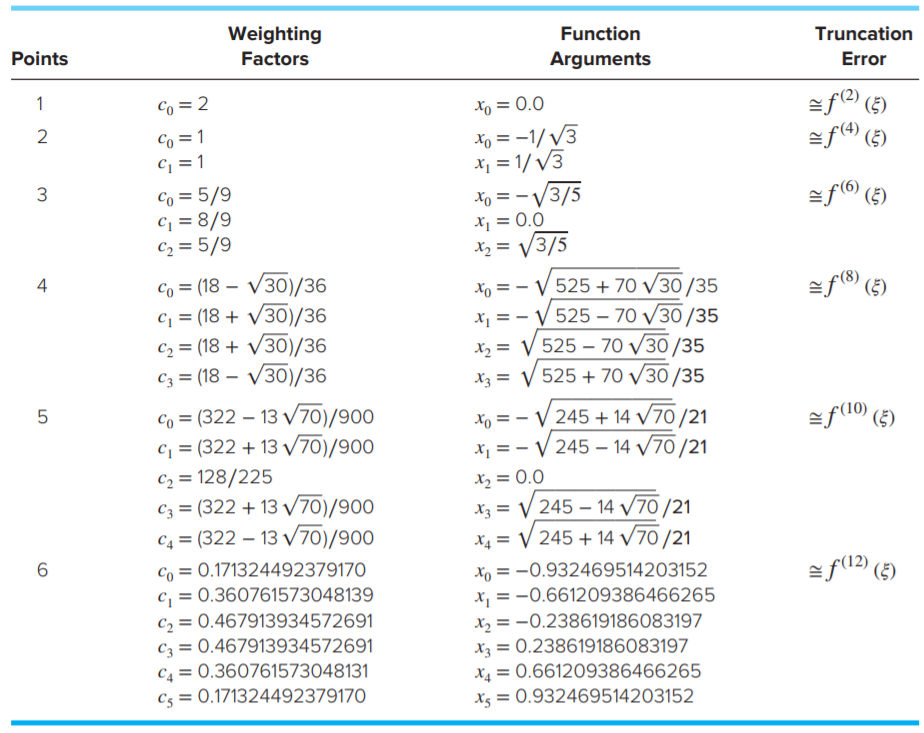
\includegraphics[width=.8\textwidth]{Integration}
	\end{figure}
	Write a function \texttt{GaussLegendre} that takes as an input
	\begin{itemize}
		\item the number of Gauss-Legendre points to be used, $n$ 
		\item a pointer to the function $f$
	\end{itemize}
	\texttt{GaussLegendre(int n, double (*f)(double(x)))}\\
	Your function should \textbf{Return} the integral approximate, $I$.
	
\end{enumerate}
\newpage
\begin{enumerate}[(b)]
	\item Test your code using the function
	$$f(y) =  0.2+25y-200y^2+675y^3-900y^4+400y^5$$
	between the limits $y=0$ to $0.8$. The exact value of the integral is $1.640533333333341$ .\\\vspace{10pt}
	NOTE: Before we can approximate this function, we have to perform a change in variable so that the limits are from -1 to 1. To do this, we substitute $a = 0$ and $b= 0.8$ into the equation
	$$ y = \frac{(b+a)+(b-a)x}{2} =0.4-0.4x$$
	and 
	$$ dy = \frac{b-a}{2}dx = 0.4dx$$
	Our equation becomes
	$$f(x) = 0.4 \bigg(0.2+25(0.4-0.4x)-200(0.4-0.4x)^2+675(0.4-0.4x)^3-900(0.4-0.4x)^4+400(0.4-0.4x)^5\bigg)$$ 
	Using your code, fill in the table below.
	
	\begin{table}[H]
		\centering
		\begin{tabular}{|c | c | c|}
			\hline
			n & I & Percent relative error \\
			\hline
			1 & \qquad \qquad \qquad \qquad \qquad \qquad \qquad & \qquad \qquad \qquad \qquad \\
			2 & & \\
			3 & & \\
			4 & & \\
			5 & & \\
			6 & & \\
			\hline
		\end{tabular}
	\end{table}
\end{enumerate}
\begin{enumerate}[(c)]
	\item How might you modify your code to compute the integral to a desired tolerance?
\end{enumerate}
	

\newpage
%%%%%%%%%%%%%%%%%%%%%%%%%%%%%%%%%%%%%%%%%%%%%%%%%%%%%%%%%%%%%%%%%%%%%%%%%%%%%%%%%%%%%%%%%%%%%%
\question{4}{Your Library}
Your final library containing ALL codes listed below. Your function declarations should be identical to the ones listed below. This includes the \textbf{function name}, the \textbf{number of parameters}, and the\textbf{ order of parameters.} 
\begin{itemize}
	\item The Bisection method, \\\texttt{Bisect(double a, double b, double tol, double (*f)(double x))}
	\item Newton-Raphson method, \\\texttt{NewtonRaphson(double a, double tol, int maxit, double (*f)(double x), double (*df)(double x))}
	\item Golden-Section Search Method, \\\texttt{GoldenSectionSearch(double xl, double xu, double tol, double (*f)(double x), bool min)}
	\item Parabolic Interpolation, \\\texttt{ParabolicInterpolation(double x1, double x2, double x3, double tol, double (*f)(double x))}
	\item The Recursive Trapezoid Rule for functions, \\\texttt{CompositeTrapezoid(double a, double b, int n, double avgdf2, double tol, double (*f)(double x))}
	\item Recursive Simpson's 1/3 Rule for functions, \\\texttt{CompositeSimpsons13(double a, double b, int n, double avgdf4, double tol, double (*f)(double x))}
	\item Simpson's Rules for data, \\\texttt{DataSimpsons(double x[], double fx[], int n)}
	\item Trapezoid Rule for data, \\\texttt{DataTrapezoid(vector<double> x, vector<double> fx, int n)}
	\item The Secant method \\\texttt{Secant(double x0, double x1, double tol, int maxit, double(*f)(double x))}
	\item Gauss Quadrature \\\texttt{GaussLegendre(int n, double (*f)(double(x)))}
	\item Forward finite difference \\\texttt{ForwardDifference(double x, double h, double (*f)(double x)}
\end{itemize}
\newpage
\begin{itemize}
	\item Backward finite difference \\\texttt{BackwardDifference(double x, double h, double (*f)(double x))}
	\item Centered finite difference \\\texttt{CenteredDifference(double x, double h, double (*f)(double x))}
\end{itemize}

\end{document}
